\documentclass[final]{beamer}

% ====================
% Packages
% ====================

\usepackage[T1]{fontenc}
\usepackage{lmodern}
\usepackage[size=custom,width=84,height=119,scale=1.0]{beamerposter}
\usetheme{gemini}
\usecolortheme{mit}
\usepackage{graphicx}
\usepackage{booktabs}
\usepackage{tikz}
\usepackage{pgfplots}
\pgfplotsset{compat=1.14}
\usepackage{anyfontsize}
\usepackage[version=4]{mhchem}
\usepackage{siunitx}
\DeclareSIUnit\bar{bar}

\graphicspath{{/home/dsimonne/Documents/Figures/}}

% ====================
% Lengths
% ====================

% If you have N columns, choose \sepwidth and \colwidth such that
% (N+1)*\sepwidth + N*\colwidth = \paperwidth
\newlength{\sepwidth}
\newlength{\colwidth}
\setlength{\sepwidth}{0.025\paperwidth}
\setlength{\colwidth}{0.3\paperwidth}

\newcommand{\separatorcolumn}{\begin{column}{\sepwidth}\end{column}}

% ====================
% Title
% ====================

\title{Multi-Scale Imaging of Corrosion and Hydrogen Embrittlement in Irradiated Nuclear Materials }

\author{David Simonne\inst{1}, \and Riley Hultquist\inst{1}, \and Sayantan Mondal\inst{1}, \and Anthony Guttiérez\inst{1}, \and Andrea Resta\inst{2}, \and Wojciech Roseker\inst{3}, \and Marilyn Sarkis\inst{4}, \and Jiangtao Zhao \inst{4}, \and Ericmoore Jossou\inst{1}}

\institute[shortinst]{\inst{1} Massachusetts Institute of Technology - USA, \inst{2} Synchrotron SOLEIL - France, \inst{3} Deutsches Elektronen-Synchrotron - Germany, \inst{4} The European Synchrotron - France}

% ====================
% Footer (optional)
% ====================

\footercontent{
  \href{https://github.com/DSimonne/PosterMRS2025}{github.com/DSimonne/PosterMRS2025}\hfill
  Material Research Society 2025, Seattle, USA \hfill
  \href{mailto:dsimonne@mit.edu}{dsimonne@mit.edu}}

% ====================
% Logo (optional)
% ====================

% use this to include logos on the left and/or right side of the header:
%\logoleft{\includesvg[height=5cm]{Figures/Logos/NSE_sub-brand_lockup_two-line_rgb_black.svg}}
% \logoright{\includesvg[height=5cm]{Figures/Logos/mit_lockup_std-three-line_rgb_mit-red.svg}}

% ====================
% Body
% ====================

\begin{document}

\begin{frame}[t]
\begin{columns}[t]

% ============================================
% First column, Introduction
% ============================================

\separatorcolumn

\begin{column}{\colwidth}

    \begin{exampleblock}{Environments in nuclear systems}

        \heading{Ten percent of the world electricity is produced \textit{via} nuclear reactors, in which structural components are exposed to an aggressive and complex environment over decades.}

        \begin{itemize}
            \setlength\itemsep{1em}
            \item Neutron radiation leads to atomic displacement / defects / dislocations.
            \item High temperature (\qty{\approx 350}{\degreeCelsius}) and high coolant pressure (\unit{\mega\pascal}).
            \item Mechanical stress, vibrations.
            \item Corrosive aqueous environment, radiolysis product / nuclear reactivity controlled with additives.
            \item \textbf{Effects can take between minutes and years to manifest.}
        \end{itemize}

    \end{exampleblock}

    \begin{block}{Radiation damage, corrosion and embrittlement}

        \begin{figure}
            \centering
            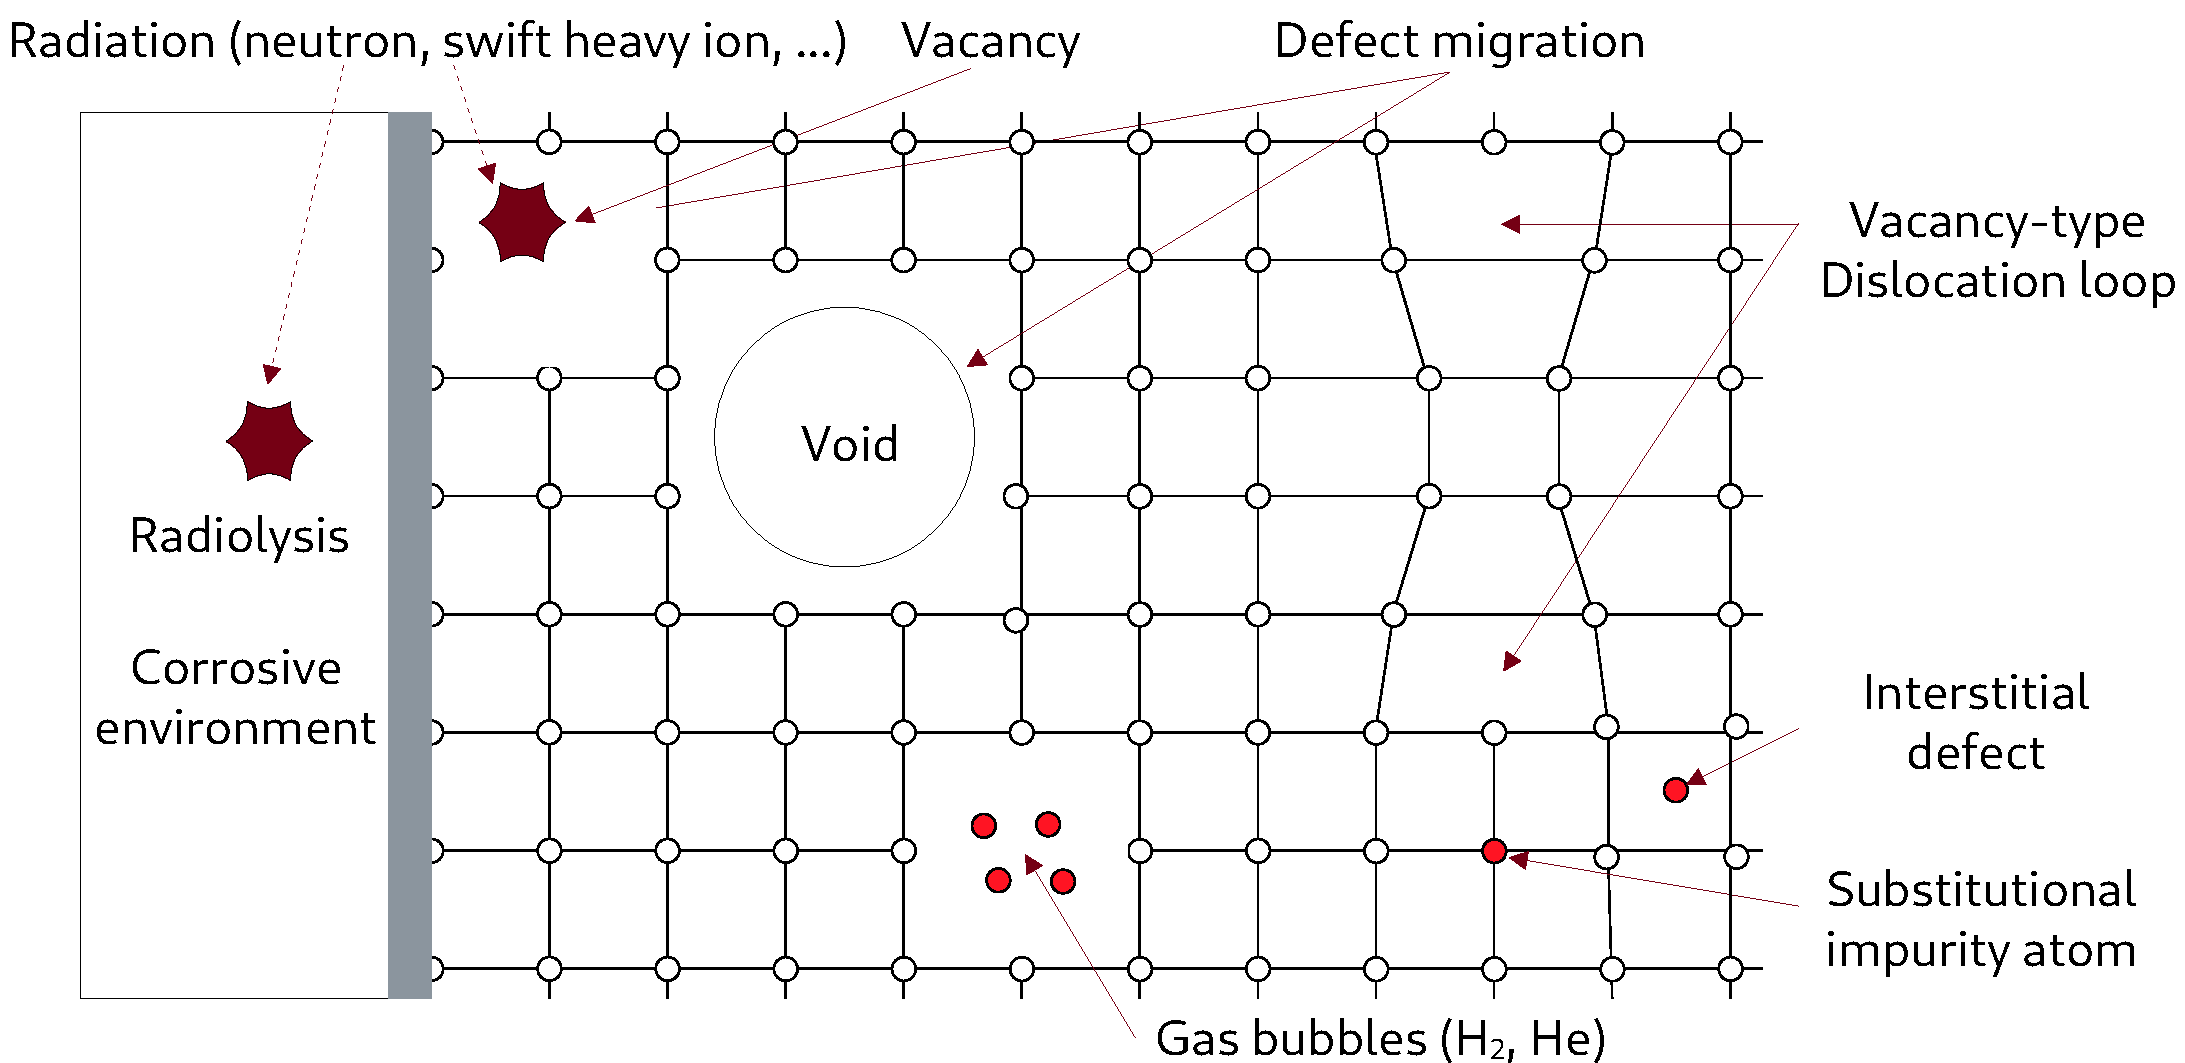
\includegraphics[width=\colwidth]{IntroductionMIT/RadiationDefects.pdf}
            \caption{Neutrons can displace atoms, creating a variety of defects.}
            \label{fig:DefectsLattice}
        \end{figure}

    \end{block}

    \begin{block}{Which materials are present?}

        \begin{columns}[T]
            \begin{column}{0.5\colwidth}

                \heading{Large variety of alloys.}

                \begin{itemize}
                    \setlength\itemsep{1em}
                    \item Pressure vessel: ferritic steel.
                    \item Corrosion resistant passivating layer: Ni-based alloys, Ni-Fe-Cr alloys, stainless steels.
                    \item Fuel cladding: zirconia alloys.
                \end{itemize}

            \end{column}

            \begin{column}{0.5\colwidth}

                \begin{figure}
                   \centering
                   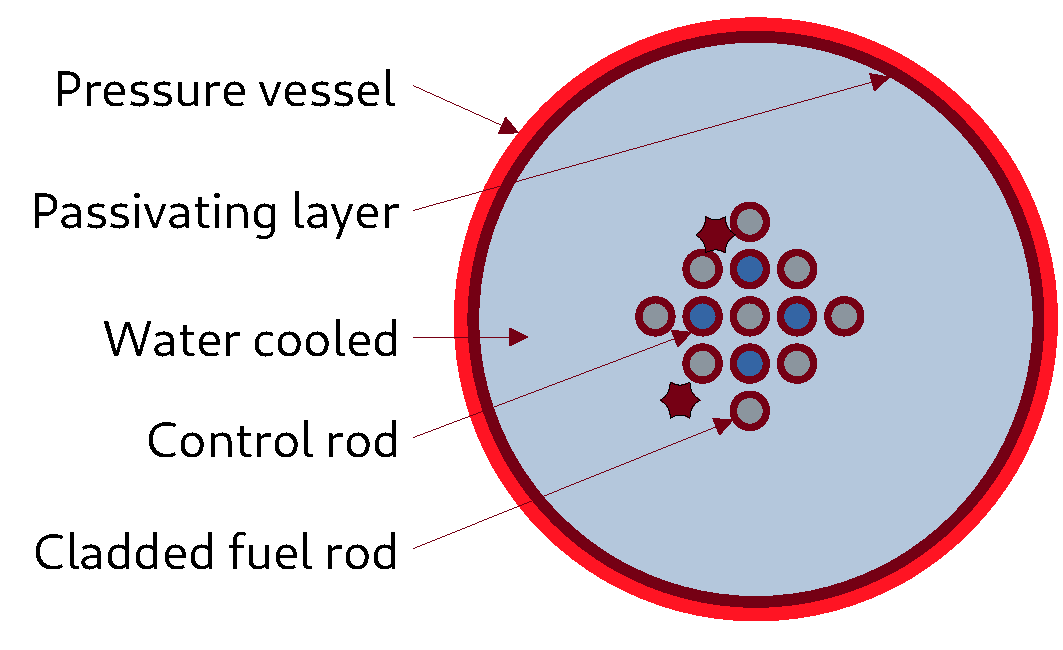
\includegraphics[width=0.49\colwidth]{IntroductionMIT/Vessel.pdf}
                   \caption{Light water reactor schematic.}
                   \label{fig:LWR}
                \end{figure}

            \end{column}
        \end{columns}

    \end{block}

    \begin{block}{Defect control}

        \heading{Heavy ion irradiation can reproduce neutron irradiation effects.}

        \begin{itemize}
            \setlength\itemsep{1em}
            \item Before / after irradiation.
            \item Ion of different nature -> interstitial defects.
            \item Ion nature, fluence and energy \rightarrow damage depth profile.
            \item We have a nuclear reactor \& an ion accelerator.
        \end{itemize}

        \begin{figure}
            \centering
            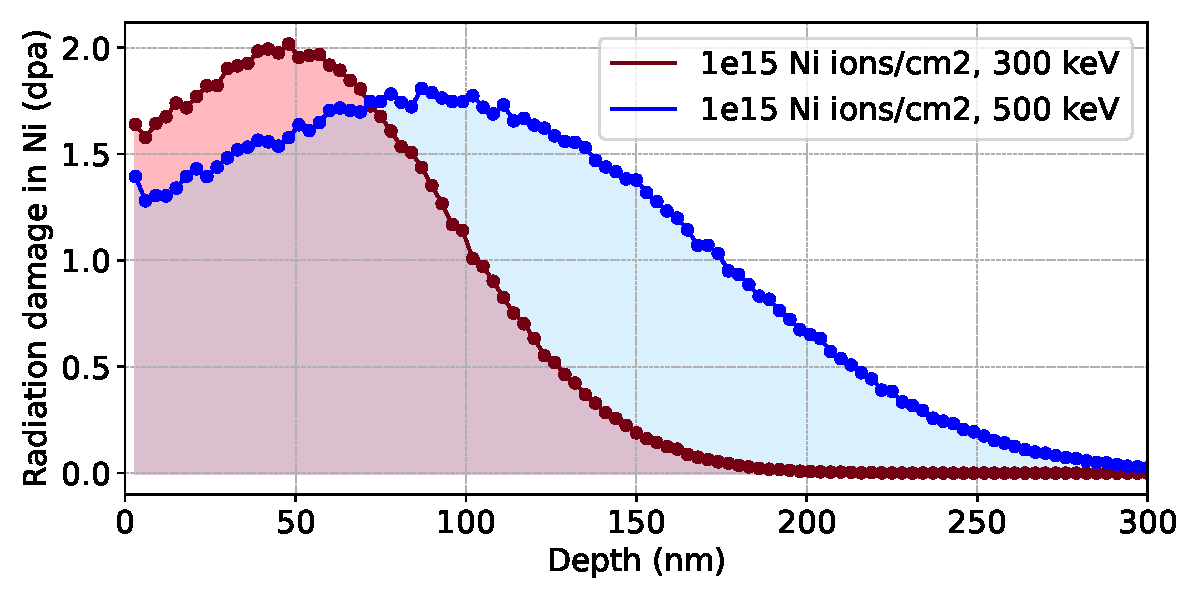
\includegraphics[width=\colwidth, trim=0 10 0 5, clip]{Radiation/NiSingleCrystals/Figures/500keV_and_300keV_DPA_damage_transfer.pdf}
            \caption{Ni ion radiation damage profile, computed with SRIM.}
            \label{fig:NiIonDamage}
        \end{figure}

        \heading{Nano-indentation allows dislocation studies.}

        \begin{itemize}
            \setlength\itemsep{1em}
            \item Before / after dislocation introduction.
            \item Dislocation type, role and mobility characterisation.
        \end{itemize}

    \end{block}

    \begin{alertblock}{Synchrotron radiation for \textit{operando} studies}

        \centering
        \begin{enumerate}
            \setlength\itemsep{1em}
            \item How does neutron radiation affect structural materials?
            \item How to measure the material's structural evolution in a \textbf{relevant} coupled environment?
            % \item Can we use radiation to stabilise some systems?
        \end{enumerate}

        \bigskip
        Standard imaging techniques do not yet offer a combined access to \textbf{operando} and \textbf{high resolution} setups.

        \bigskip
        Synchrotron radiation provides intense, coherent, focused, and tunable X-rays that allow us to work in complex environments!

    \end{alertblock}

\end{column}

% ============================================
% Second column, Techniques and samples
% ============================================

\separatorcolumn

\begin{column}{\colwidth}

    \begin{alertblock}{Measuring strain in three dimensions}

        Bragg Coherent Diffraction Imaging relies on:

        \begin{itemize}
            \setlength\itemsep{1em}
            \item Highly coherent synchrotron sources.
            \item Samples below coherent volume: \qty{\approx 1}{\um^3}.
            % \item The beam must be very intense and focused since the samples are very small.
            % \item High setup stability, possibility to go probe high angles, in many different directions.
            \item Highly faceted samples.
        \end{itemize}

        \begin{figure}
            \includegraphics[width=0.45\textwidth]{/IntroductionMIT/BraggLaw.png}
            \includegraphics[width=0.45\textwidth]{/IntroductionMIT/StrainedCrystal.png}
        \end{figure}

        \centering
        Access to \textbf{full displacement field} \textrightarrow Defect identification!

    \end{alertblock}

    \begin{block}{Sample preparation}

        \begin{columns}[T]
            \begin{column}{0.6\colwidth}
                \begin{figure}
                    \centering
                    \includegraphics[width=0.575\colwidth]{MITSamples/Char/SEM/SEM_Poster.pdf}
                    \caption{EBL pattern and Ni particles imaged by scanning electron microscopy.}
                    \label{fig:EBLPattern}
                \end{figure}
            \end{column}

            \begin{column}{0.4\colwidth}
                \begin{enumerate}
                    \item Pattern drawn by electron beam lithography (EBL).
                    \item Crystallization by annealing in forming atmosphere.
                    \item SEM imaging and EBSD crystal orientation determination.
                \end{enumerate}

            \end{column}

        \end{columns}

    \end{block}

    \begin{block}{Sample characterisation}

        \heading{The interface plays a crucial role in the supported crystals shape, orientation, and strain field.}

        \begin{table}[htb]
            \centering
            \resizebox{\textwidth}{!}{%
                \begin{tabular}{@{}lllllll@{}}
                \toprule
                Substrate  & \ce{Nb}:\ce{SrTiO3}(001) & \ce{SiO2}(001)(1 ML)& \ce{SiO2}(001)(2 ML)& \ce{SiO2}(001)( 3ML)& \ce{SiO2}(001) & Si(001) \\
                 &  & /Si(001) & /Si(001) & /Si(001) &  & \\
                \midrule
                $W_{\text{sep}}$ (\unit{\J/\meter^2})  & 0.19 & 0.61 & 0.70 & 1.60 & 2.16 & 3.16 \\
                 $\gamma_{int}$ (\unit{\J/\meter^2})  & 2.76 & -- & -- & -- & 2.92 & 0.97 \\
                 \bottomrule
                \end{tabular}%
            }
            \caption{Work of separation $W_{\text{sep}}$ and interfacial energies ($\gamma_{int}$) for Ni(111) on different substrates.}
            \label{tab:wos_gamma_table}
        \end{table}

        \begin{figure}
            \centering
            \includegraphics[width=\colwidth]{MITSamples/Char/TEM/TEM_DFT.pdf}
            \caption{a) Cross-sectional TEM image of a Ni particle on \ce{SiO2} / \ce{Si}(001) substrate.
            b) Zoom on interphase boundary with c) EDS measurement and d) Interface schematic. e) DFT cell used for interface calculations in Tab. \ref{tab:wos_gamma_table}.}
        \end{figure}

        \begin{figure}
            \centering
            \includegraphics[width=\colwidth]{MITSamples/Char/SXRD/InPlaneMaps.pdf}
            \caption{
            In-plane reciprocal space maps of Ni dewetted on \ce{SiO2} covered [001] oriented \ce{Si} (left), and [001] oriented \ce{Nb}:\ce{SrTiO3} (right).
            }
        \end{figure}

    \end{block}

    \begin{block}{\textit{In situ} corrosion cell}
        \begin{figure}
            \centering
            \includegraphics[width=0.9\colwidth]{/ElectrochemicalCell/Fig_ABCD.pdf}
            \caption{Electrochemical cell design, compatible with three electrode setup, liquid flow, and four different synchrotron beamlines.}
        \end{figure}
    \end{block}

\end{column}

% ============================================
% Third column, Results, key takeaways, references,
% acknowledgments
% ============================================

\separatorcolumn

\begin{column}{\colwidth}

    \begin{block}{X-ray irradiation strain relaxation effect}
        \begin{figure}
            \centering
            \includegraphics[width=\colwidth]{BeamEffect/Si_G/Si_G_Beam_effect_Poster.pdf}
            \caption{Strain relaxation of a Ni particle on \ce{SiO2}/\ce{Si}(001) from highly fluent X-ray beam visible by Bragg peak assymetry (top) and strain field (middle).
            The strain field energy (bottom) presents a quantitative decrease of the strain field inside the particle.
            }
        \end{figure}
    \end{block}

    \begin{block}{Corrosion in light water reactor environment}
        \begin{figure}
            \centering
            \includegraphics[width=\textwidth]{Corrosion/NiCo/MRSPoster.pdf}
            \caption{Strain buildup during corrosion of NiCo particle.}
        \end{figure}
    \end{block}

    \begin{block}{Defect signature in X-ray microscopy}
        \heading{Dark-field X-ray microscopy enables the visualisation of crystalline defects over extended ranges.}

        \begin{figure}
            \centering
            \includegraphics[width=\textwidth]{DFXM/Poster.pdf}
            \caption{DFXM image of Fe single crystal. Dislocations are visible over several hundreds of micrometers before hydrogen embrittlement.}
        \end{figure}
    \end{block}

    % \begin{block}{Scientific vision}
    %     \includegraphics[width=0.9\colwidth]{IntroductionMIT/Overall-research-vision.jpg}
    % \end{block}

    \begin{alertblock}{Key takeaways}
        \begin{itemize}
            \setlength\itemsep{1em}
            \item Synchrotron radiation allows \textit{operando} studies.
            \item Strain signature is accessible \textit{via} Bragg imaging techniques.
            \item Combining techniques allows nano as well as meso scale information.
        \end{itemize}

        \heading{Multi-scale approach, sensitive to material density, crystal structure, and defects, during \textit{operando} studies.}

    \end{alertblock}

    \begin{block}{References}
        \nocite{*}
        \footnotesize{\bibliographystyle{abbrv}\bibliography{references}}
    \end{block}

    \begin{block}{Acknowledgments}
        \centering
        \footnotesize{
            This work was funded by the Faculty Startup Fund support from MIT.
            The sample preparation work was carried out in part at MIT.nano, thanks to the help of Dr. Aubrey Penn and Juan Fererra.
            We acknowledge the ESRF and SOLEIL synchrotrons in France for providing beamtime utilizing beamline ID01 and SixS.
            We used the HPC at INL, supported by the Office of Nuclear Energy of the U.S. DOE and the NSUF under Contract No. DE-AC07-05ID14517.
        }

        \bigskip

        
\includegraphics[height=2.5cm]{Logos/NSE/NSE_sub-brand_lockup_two-line_rgb_black.png}

    \end{block}

\end{column}

\separatorcolumn

\end{columns}
\end{frame}

\end{document}
